\documentclass{beamer}
\usepackage[utf8]{inputenc}
\usepackage{default}
\usepackage{multirow} 
\usepackage{amsmath} 
\usepackage{listings}
\lstset{ %
                % choose the language of the code
basicstyle=\footnotesize,       % the size of the fonts that are used for the code
numbers=left,                   % where to put the line-numbers
numberstyle=\footnotesize,      % the size of the fonts that are used for the line-numbers
stepnumber=1,                   % the step between two line-numbers. If it is 1 each line will be numbered
numbersep=5pt,                  % how far the line-numbers are from the code
backgroundcolor=\color{white},  % choose the background color. You must add \usepackage{color}
showspaces=false,               % show spaces adding particular underscores
showstringspaces=false,         % underline spaces within strings
showtabs=false,                 % show tabs within strings adding particular underscores
frame=single,           % adds a frame around the code
tabsize=2,          % sets default tabsize to 2 spaces
captionpos=b,           % sets the caption-position to bottom
breaklines=true,        % sets automatic line breaking
breakatwhitespace=false,    % sets if automatic breaks should only happen at whitespace
escapeinside={\%*}{*)}          % if you want to add a comment within your code
}

\usetheme{Berkeley}

\title{Subprogramas}
\author{Guilherme, Gustavo, Sean e Vinícius}
\institute{Universidade Estadual de Londrina}

\begin{document}

\frame{\titlepage}
\frame {
\frametitle{Sumário}
\tableofcontents
}

%!TEX root = slide.tex

\section{Subprogramas Como Parâmetro}
\begin{frame}{Subprogramas Como Parâmetro}
	\begin{itemize}
	  \item Ideia simples, mas gera complicações.
	  \item \emph{Type checking}.
	  \item referencing environment.
	\end{itemize}
\end{frame}

\begin{frame}{Referencing Environment}
	\begin{itemize}
	  \item Linguagens que permitem subprogramas aninhados.
	  \item Shallow Binding
	  \item Deep Binding
	  \item Ad Hoc Binding
	\end{itemize}
\end{frame}

\begin{frame}{Exemplo}
	\begin{figure}[ht!]
		\centering
		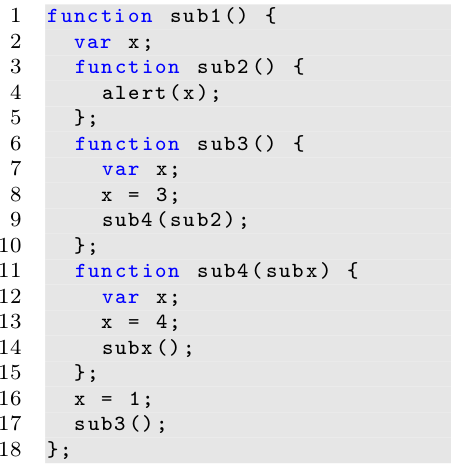
\includegraphics[scale=0.4]{./imgs/js-original}
	\end{figure}
\end{frame}

\begin{frame}{Shallow Binding}
	O ambiente é o local onde o subprograma é chamado.
\end{frame}

\begin{frame}{Shallow Binding}
	\begin{figure}[ht!]
		\centering
		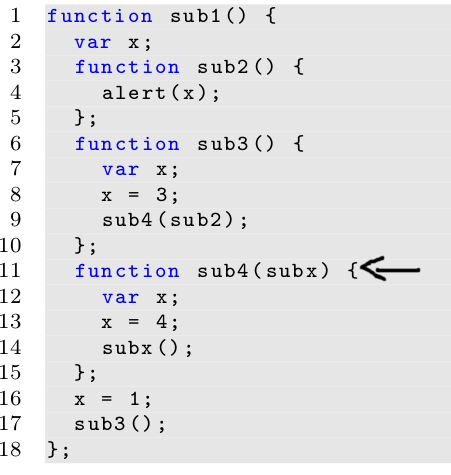
\includegraphics[scale=0.4]{./imgs/js-shallow}
	\end{figure}
\end{frame}

\begin{frame}{Deep Binding}
	O ambiente refere-se onde o subprograma foi definido.
\end{frame}

\begin{frame}{Deep Binding}
	\begin{figure}[ht!]
		\centering
		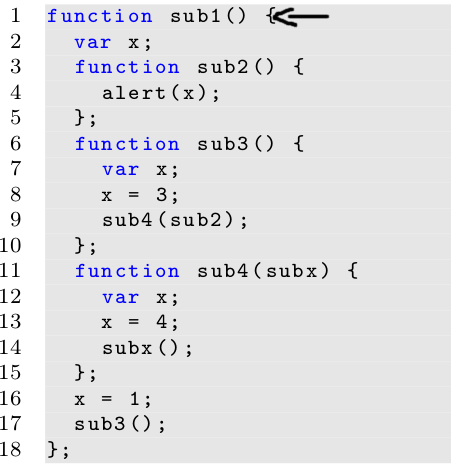
\includegraphics[scale=0.4]{./imgs/js-deep}
	\end{figure}
\end{frame}

\begin{frame}{Ad Hoc Binding}
	O ambiente condiz com o local que o subprograma foi passado por parâmetro.
	Nunca implementado.
\end{frame}

\begin{frame}{Ad Hoc Binding}
	\begin{figure}[ht!]
		\centering
		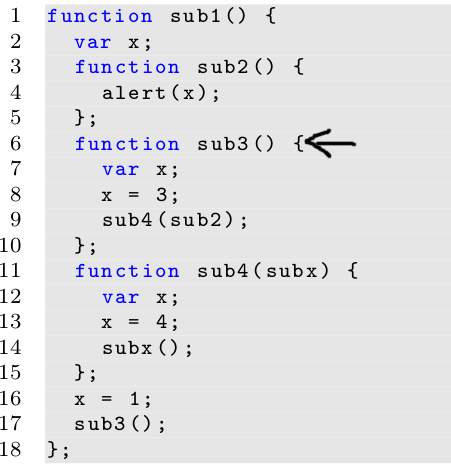
\includegraphics[scale=0.4]{./imgs/js-adhoc}
	\end{figure}
\end{frame}

\section{Chamar Subprogramas Indiretamente}
\begin{frame}{Chamar Subprogramas Indiretamente}
	\begin{itemize}
	  \item Subprograma conhecido em tempo de execução.
	  \item GUI e callback.
	  \item C/C++ ponteiro para função.
	  \item C\# Delegate.
	\end{itemize}
\end{frame}

\begin{frame}[fragile]{C/C++ - Ponteiro Para Função}
	\begin{lstlisting}[language=c]
		//declaracao da funcao
		int sum(int a, int b)
		{
			return a + b;
		}

		//ponteiro para a funcao
		int (*sum_pointer)(int, int);
		sum_pointer = &sum;
		
		//chamar a funcao
		(*sum_pointer)(1,2);
	\end{lstlisting}
\end{frame}

\begin{frame}[fragile]{C\# - Delegate}
	\begin{lstlisting}[language=csh]
		//declarar um delegate
		public delegate int SumDelegate(int a, int b);
		...
		//instanciar um delegate (funcao sum tem a mesma assinatura)
		SumDelegate sumDelegate = new SumDelegate(sum);
		//executar
		sumDelegate(2,3);
	\end{lstlisting}
\end{frame}

\section{Sobrecarga de Subprogramas}
\begin{frame}{Sobrecarga de Subprogramas}
	\begin{itemize}
	  \item Subprogramas (diferentes) com o mesmo nome.
	  \item Parâmetros diferentes.
	  \item Subprogramas relacionados.
	  \item Exemplo: Sobrecarga de construtor.
	  \item Ada, Java, C++, C\# e F\#.
	\end{itemize}
\end{frame}

\section{Suprogramas Genéricos}
\begin{frame}{Suprogramas Genéricos}
	\begin{itemize}
	  \item Reuso de software é algo importante.
	  \item Subprogramas com tipos genéricos.
	  \item Exemplo: Ordenação independente de tipo.
	  \item C++ - Templates
	  \item Java e C\# - Generics
	\end{itemize}
\end{frame}

\begin{frame}[fragile]{C++ - Templates}
	\begin{lstlisting}[language=c++]
		//declarar funcao template
		template <class myType>
			myType GetMax (myType a, myType b) {
			return (a>b?a:b);
		}
		...
		//exemplo de chamada para inteiro
		GetMax<int> (1,2);
		...
		//exemplo de chamada para float
		GetMax<float> (1,2);
	\end{lstlisting}
\end{frame}

\begin{frame}[fragile]{Java - Generics}
	\begin{lstlisting}[language=Java]
		//declarar um metodo generico.
		public static <T> T doIt(T[] list) {
			...
		}
		...
		//chamar o metodo para String
		doIt<String>(myList);
		
		...
		//chamar o metodo para Integer
		doIt<Integer>(myList);
		
		...
		//isso causaria um erro (tipo primitivo)
		doIt<int>(myList);
	\end{lstlisting}
\end{frame}

\end{document}
